%generare il pdf con il comando: pdflatex main.tex
\documentclass[a4paper, oneside, openany,12pt]{article}
\usepackage{graphbox}
% permette di modificare i margini
\usepackage[top=3.1cm, bottom=3.1cm, left=2.2cm, right=2.2cm]{geometry}
\usepackage{lastpage} %info sul # dell'ultima pagina del documento
\usepackage{fancyhdr} %per modificare dimensioni,margini, intestazioni e righe a piè di pagina

\usepackage[htt]{hyphenat}

\fancypagestyle{plain}{
  % cancella tutti i campi di intestazione e piè di pagina
  \fancyhf{}
  
  \rhead{\sectiontitle}
  
  \rfoot{Page \thepage{} di \pageref{LastPage}} %es: pag: 4 di 10

  %linea orizzontale alle posizioni top e bottom della pagina
  \renewcommand{\headrulewidth}{0.2	pt}  
  \renewcommand{\footrulewidth}{0.2pt}
}
\pagestyle{plain}

%Comando Spazio
\newcommand{\Spazio}{\mbox{} \\ \mbox{} \\ }  


%\usepackage{calc} %introduce la notazione infissa per le op. aritmetiche interne a LaTeX

\usepackage[utf8]{inputenc}
\usepackage[T1]{fontenc}
\usepackage[english]{babel} %il documento è in inglese
%\usepackage{textcomp} %The pack­age sup­ports the Text Com­pan­ion fonts, which pro­vide many text sym­bols
%(such as baht, bul­let, copy­right, mu­si­cal­note, onequar­ter, sec­tion, and yen), in the TS1 en­cod­ing.

\usepackage{graphicx}       %permette di inserire delle immagini
\usepackage{caption}        %numerazione figure e loro descrizione testuale
\usepackage{subcaption}     %sottofigure numerabili
\usepackage{float}  %permette di inserire un # qualsiasi di figure fluttuanti
\usepackage{xcolor}
\usepackage{color, colortbl}
\usepackage{rotating} %permette di ruotare le immagini
%\usepackage{changepage} %utile se c'è bisogno di aggiustare margini per centrare figure

%package utili per la math mode ( $ ... $ o \[ ... \] )
\usepackage{amsmath}
\usepackage{amssymb}
\usepackage{amsfonts}
%\usepackage{euler}    %font 'ams euler', lo stesso di 'Concrete Mathematics' di Knuth
\usepackage{amsthm}
\usepackage{mathtools}

% package utili per tabelle(\thead in particolare)
\usepackage{array, booktabs, caption}
\usepackage{makecell}
\renewcommand\theadfont{\bfseries}
\usepackage{boldline}

\usepackage{listings} %permette di inserire degli spezzoni di codice

\usepackage{tikz} %disegno di immagini vettoriali a schermo. Utile per grafi
\usetikzlibrary{arrows.meta}
\usetikzlibrary{graphs}
\usetikzlibrary{arrows}
%\usepackage{tikz-uml} %serve per disgnare l'UML, fantastica guida:
%https://perso.ensta-paristech.fr/~kielbasi/tikzuml/var/files/doc/tikzumlmanual.pdf
%download package: http://perso.ensta-paristech.fr/~kielbasi/tikzuml/

%package per le tabelle
\usepackage{booktabs} %permette di poter usare delle liste nelle tabelle
\usepackage{tabularx} 
\usepackage{longtable} %una tabella può continuare su più pagine
\usepackage{multirow} %utile per visualizzare una cella su più righe
%\usepackage{multicolumn} %cella su più colonne
%\usepackage[table]{xcolor} %rende disponibile l'utilizzo di un colore per lo sfondo
                        %delle celle di una tabella

%crea una cella per le tabelle in grado di andare a capo con \newline
%https://tex.stackexchange.com/questions/12703/how-to-create-fixed-width-table-columns-with-text-raggedright-centered-raggedlef
\usepackage{array}
\newcolumntype{L}[1]{>{\raggedright\let\newline\\\arraybackslash\hspace{0pt}}m{#1}}
\newcolumntype{C}[1]{>{\centering\let\newline\\\arraybackslash\hspace{0pt}}m{#1}}
\newcolumntype{R}[1]{>{\raggedleft\let\newline\\\arraybackslash\hspace{0pt}}m{#1}}


%indice con i puntini
\usepackage{tocloft}
\renewcommand\cftsecleader{\cftdotfill{\cftdotsep}}

%Pacchetto per i colori delle tabelle
\usepackage{color, colortbl}

%http://ctan.mirror.garr.it/mirrors/CTAN/macros/latex/contrib/appendix/appendix.pdf
\usepackage{appendix} %aggiunge dei comandi per l'appendice
\usepackage{parskip} %aiuta LaTeX a trovare il miglior stile per i page break
\setcounter{secnumdepth}{5} % numera i sottoparagrafi
\setcounter{tocdepth}{5} %aggiunge all'indice i sottoparagrafi
%\usepackage{titlesec} %\begin{paragraph} si può usare come subsubsubsection!


\usepackage{breakurl}%\url{...} può continare alla linea successiva. (si può andare a capo)

\definecolor{Maroon}{cmyk}{0, 0.87, 0.68, 0.32}
\usepackage[colorlinks=true]{hyperref}
\hypersetup{
    colorlinks=true,
    citecolor=black,
    filecolor=black,
    linkcolor=black, % colore dei link interni
    urlcolor=blue  % colore dei link interniesterni
}

%impostazioni per il codice che deve finire dentro a
%\begin{lstlisting}

\definecolor{listinggray}{gray}{0.9}
\definecolor{lbcolor}{rgb}{0.9,0.9,0.9}
\lstset{
backgroundcolor=\color{lbcolor},
    tabsize=4,    
%   rulecolor=,
    language=[GNU]C++,
    basicstyle=\scriptsize,
    upquote=true,
    aboveskip={1.5\baselineskip},
    columns=fixed,
    showstringspaces=false,
    extendedchars=true,
    inputencoding=utf8,
    breaklines=true,
    prebreak = \raisebox{0ex}[0ex][0ex]{\ensuremath{\hookleftarrow}},
    frame=single,
    numbers=left,
    showtabs=false,
    showspaces=false,
    showstringspaces=false,
    identifierstyle=\ttfamily,
    keywordstyle=\color[rgb]{0,0,1},
    commentstyle=\color[rgb]{0.026,0.112,0.095},
    stringstyle=\color[rgb]{0.627,0.126,0.941},
    numberstyle=\color[rgb]{0.205, 0.142, 0.73},
%        \lstdefinestyle{C++}{language=C++,style=numbers}’.
}
\lstset{
  backgroundcolor=\color{white},
  tabsize=4,
  language=C++,
  captionpos=b,
  tabsize=3,
  frame=lines,
  numbers=left,
  numberstyle=\tiny,
  numbersep=5pt,
  breaklines=true,
  showstringspaces=false,
  basicstyle=\footnotesize,
  identifierstyle=\color{black},
  keywordstyle=\color[rgb]{0,0,1},
  commentstyle=\color{gray},
  stringstyle=\color{red}
}
% Creazione della copertina
\newcommand{\copertina}{
  \newgeometry{top=5cm}
  
  \begin{titlepage}
  \begin{center}
 
	\begin{tikzpicture}[remember picture, overlay, scale=.5, transform shape, opacity=0.15]
		\node[anchor=center] at (current page.west){%
		\pgfimage{Style/logo.png}};
	\end{tikzpicture}
    
  \vspace{1cm}

  \begin{Huge}
    \textbf{Advanced Algorithms}\\
    \vspace{20pt}  
    \textbf{Assignment 2:} \\
    \textbf{Traveling Salesman Problem} \\
  \end{Huge}

  \vspace{9pt}  
  
  \begin{large}
  	\today
  \end{large}	  
  
  \vspace{15pt}
  
  \vspace{15pt}

  \begin{center}
  	
  	\begin{tabular}{ c c }
		\textbf{Budai Matteo} & 2057217  \\
		\textbf{Burke Jamie} & 2044062 \\
		\textbf{Tlepin Sanjar} & 2041606  \\
  	\end{tabular}
  	
  \end{center}

  \end{center}
  \end{titlepage}
  
  \restoregeometry
}

\newcommand{\code}[1]{\flextt{\texttt{#1}}}

\newcommand{\gl}[1]{\textit{#1}\ped{g}}

\newcommand{\sectiontitle}{}



\begin{document}
\copertina
\tableofcontents
\pagebreak

%\listoffigures
%\listoftables

% Comando per testare con le linee più grosse
\arrayrulewidth=1pt
% Colori per la tabella
\definecolor{title_row}{rgb}{0.13, 0.59, 0.95}
\definecolor{title_text}{rgb}{1, 1, 1}

% SEZIONI DEL DOCUMENTO
% qui vanno presentate in ordine di apparizione le sezioni che compongono il documento
\input{Res/Sections/introduction.tex}
\section{Neirest Neighbor Algortihm}\label{neirest}


\subsection{Input and Data Structures}


\subsection{Implementation}


\subsection{Complexity}


\pagebreak
\section{Random Insertion Algorithm}\label{randominsertion}
Idea of the algorithm is to take randomly a node and find the cheapest path going through that random k from pair of nodes in our partial circuit. 
As it was mentiond erlier, the graph initialization functions create graph as a list of edges and also provide us a list of all nodes.
The Implementation of the code follow the based concept:

\begin{itemize}
    \item \textbf{Initialization}: Take first node (we always took first node from the graph and make it as partial circuit;
    \item \textbf{Selection}: Random select node not in partial circuit;
    \item \textbf{Insertion}: Find edge in partial circuit that minimize the triangle inequality: w(i,k)+w(k,j)-w(i,j) and insert k between i and j;
    \item \textbf{Repeat}: step \textbf{Selection} and \textbf{Insertion} until add all nodes to partial circuit.
\end{itemize}


\subsection{Functions}
We implement 3 functions: 

\begin{itemize}
	\item \textbf{RandomInsertion()}: Main function that call other in process of counting the triangle inequality and check the distance.
	\item \textbf{buildPath(p,k)}: Function to get the distance required to get to random k and also position after we need to insert. 
	\item \textbf{minDist(u)}: Function to get closest node to input one.
\end{itemize}

\subsection{Implementation}
The final solution is the following:
\begin{itemize}
	\item We start the time;
	\item We execute a deep copy unvisited of the original list v;
	\item We follow the algorithm and we start from the node 0 \textit{(startingNode)} of the unvisited list;
\end{itemize}

Originality, that we found pretty usefull in minDist function is to run in cicle of data instead of all graph.




\pagebreak
\section{2-approximate Algorithm}\label{2-approximate}
The 2-approximate algorithm starts by defining a starting node from the list of vertices within a graph, and then a minimum spanning tree is constructed using Prim's algorithm with the starting node as the root. The vertices of the MST are then visited in a preorder walk/depth first search, and added to a list in the order of which they are visited. Finally, the starting node is added at the end of the preorder list in order to complete the Hamiltonian cycle in the MST. 

\begin{lstlisting}[mathescape=true]
APPROX_METRIC_TSP (G)
    V = { $v_1,v_2, ... ,v_n$ } 
    r $\leftarrow v_1$
    $T^* \leftarrow$ PRIM (G,r)
    < $v_{i1},v_{i2}, ... ,v_{in} > = H^{ '} \leftarrow$ PREORDER ($T^{*}$, r) 
    return < $H^{'}, v_{i1}$ > = H
    
\end{lstlisting}

\subsection{Input and Data Structure}
The 2-approximate algorithm requires a minimum spanning tree to be constructed using Prim's algorithm, and in order to be efficient, Prim's algorithm requires a heap data structure. We reused Prim's algorithm and the min heap data structure that were implemented in Assignment 1 for this course; however, the input files for Assignment 1 provided a list of connected nodes, whereas the input files for Assignment 2 only provide a list of distinct vertices and their x and y coordinates. Consequently, we made the following modifications to the Graph and Node classes, and added two new functions: 
\begin{itemize}
	\item  \textbf{Node}: three new instance variables are initialized:
	    \begin{itemize}
	    \item xcoord: x-coordinate of vertex
	    \item ycoord: y-coordinate of vertex
	    \item weighttype: weight type of the vertex, either Euclidean or Geographic
	    \end{itemize}
	\item  \textbf{Graph}: the buildGraph function restructures the input file to resemble the input file format of Assignment 1, before calling the createNodes and makeNodes functions. Specifically, the buildGraph function takes each vertex and connects it to all other vertices in the input file. 
	\item  \textbf{Weight}: new function that takes the weight type, x-coordinate, and y-coordinate for two vertices as input, and returns the weight between the two vertices. For the Euclidean weight type, there is no coordinate conversion and we simply calculate the Euclidean distance rounded to the nearest integer. For the Geographic weight type, the x- and y-coordinates are converted to radians and then the geographic distance is calculated using the instructions in the FAQ site provided by the assignment.
	\item  \textbf{Preorder}: new function that takes a MST graph, starting node, and empty set as input. The vertices of the MST are visited in a preorder walk/depth first search and added to the list in that order. The list is returned once all vertices of the MST have been visited and added to the list.   
	
\end{itemize}


\subsection{Implementation}
The solution to the cost of the Hamiltonian cycle in the MST is performed in the following steps:
\begin{enumerate}
    \item Create the Graph object through the Graph() class and call the buildGraph method
    \item Calculate the MST of the graph using Prim's algorithm
    \item Call the Preorder function, passing the inputs of the MST and the same starting node used as the root in Prim's algorithm.
    \item Append the starting node to the end of the list returned by the Preorder function in order to complete the Hamiltonian cycle in the MST 
    \item Call the Weight function to calculate the distance between each node in the Hamiltonian cycle, sum all of the edge weights to calculate the total cost of the cycle
\end{enumerate}
\pagebreak
\section{Results}\label{results}

\subsection{Table of results}

	\begin{figure}[H]
		\hspace{0cm}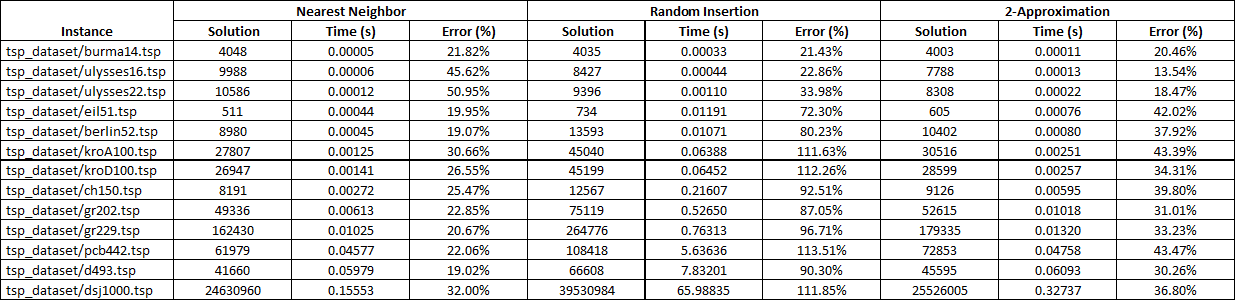
\includegraphics[width=17cm]{Img/resultstable.png}
		\caption{Table of results}
	\end{figure}

\subsection{Graph of the execution time comparison}
	
	\begin{figure}[H]
		\hspace{0cm}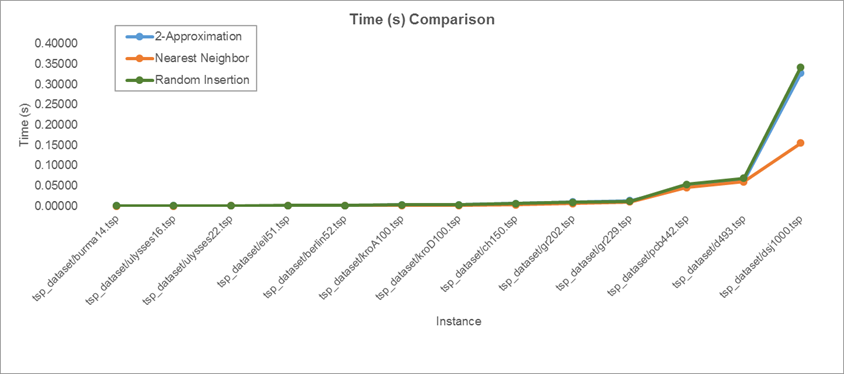
\includegraphics[width=17cm]{Img/timecomparisonchart.png}
		\caption{Execution time comparison}
	\end{figure}
	

\subsection{Graph of the error comparison}
	
	\begin{figure}[H]
		\hspace{0cm}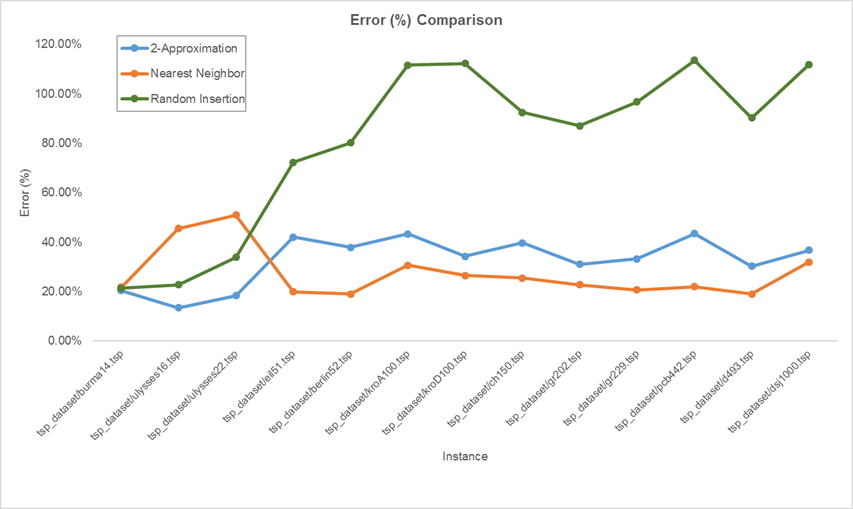
\includegraphics[width=17cm]{Img/errorcomparisonchart.png}
		\caption{Error comparison}
	\end{figure}


\pagebreak
\input{Res/Sections/conclusion.tex}


\end{document}